\documentclass[12pt,a4paper]{scrartcl}
\usepackage{url, booktabs,pdflscape}
\usepackage[final]{pdfpages}
\usepackage[colorlinks]{hyperref}
\title{Student Robotics Kickstart Risk Assessment Form}

\begin{document}
\maketitle

\begin{description}
\item[Activity being assessed:] Student Robotics Kickstart 2013 (13/10/2012)
\item[Location:] Room 1015, Building 32, Highfield Campus, University of Southampton (\url{http://data.southampton.ac.uk/building/32.html}) and Garden Court, Building 40, Highfield Campus, University of Southampton (\url{http://data.southampton.ac.uk/building/40.html})
\item[Who is exposed to the hazard:] Competitors, Team Leaders, Blueshirts
\end{description}

\begin{description}
\item[Assessor's name:]
\item[Assessor's job title:]
\item[Assessor's signature:]
\item[Date of assessment:]
\end{description}
\clearpage

\newcommand{\risk}[3]{
 #1 & #2 & #3 \\
}

\begin{landscape}
\section{Risks}
The following risks have been considered for the Student Robotics Kickstart event.  Further description of the meaning of risk ratings (presented in this section as $L \times S$) can be found in the next section.

A safety briefing will be given during the introductory talk, covering the points below.

\bigskip
\begin{tabular*}{\linewidth}[c]{p{14em}p{30em}c}
\toprule
\textbf{Hazard} & \textbf{Control Measures} & \textbf{Risk Rating} \\
\midrule

\risk{Injury while using mini-game tools and materials}
% Fill me in
{Student Robotics Blueshirts will supervise all use of tools and materials at the mini-game. Since the primary material is card and the most dangerous of the tools is scissors, Student Robotics views the risk as low.}
{1}

\risk{Electric shock by contact between water, electrical output and human}
{Water and electrical outputs kept strictly apart. Food and Drink is not allowed in clearly marked, Blueshirt-only areas.}
{3}

\risk{Risk of Fire}
{No naked flames are allowed to be used intentionally. If a fire breaks out accidentally, University of Southampton regulations will be followed as detailed below}
{2}
\bottomrule
\end{tabular*}
\end{landscape}

\begin{landscape}

\section{Assessment Guidance}

The risk ratings of the risks in the previous section are calculated by multiplying $L$, the likelihood rating, by $S$, the severity rating.

\bigskip
\begin{minipage}[b]{0.5\linewidth}
\begin{tabular}[c]{lc}
\hline
  \textbf{Likelihood} & \textbf{Likelihood rating} \\
\hline
  Very unlikely & 1 \\
  Unlikely & 2 \\
  Likely & 3 \\
  Fairly likely & 4 \\
  Very likely & 5 \\
\hline
\end{tabular}
\end{minipage}
\begin{minipage}[b]{0.5\linewidth}
\begin{tabular}[c]{lc}
\hline
  \textbf{Severity} & \textbf{Severity rating} \\
\hline
  First Aid injury/illness & 1 \\
  Minor injury/illness & 2 \\
  `3 day' injury/illness & 3 \\
  Major injury/illness & 4 \\
  Fatality/disabling injury & 5 \\
\hline
\end{tabular}
\end{minipage}
\bigskip

The following should be used to rate the risk and plan corrective action:
\bigskip
\newcommand{\riskinfo}[4]{
  #1 & #2 & #3 & #4 \\
}

\begin{tabular*}{\linewidth}[c]{cccp{33em}}
\hline
  \textbf{Risk Rating} & \textbf{Category} & \textbf{Tolerability} & \textbf{Comments} \\
\hline

  \riskinfo{1--2}{Very Low}{Acceptable}
  {No further action is necessary other than to ensure that the controls are maintained.}

  \riskinfo{3--4}{Low}{Acceptable}
  {No additional controls are required unless they can be implemented at very low cost (in terms of time, money and effort).}

  \riskinfo{5--7}{Medium}{Tolerable}
  {Consideration should be given as to whether the risks can be lowered, where applicable, to a tolerable level, and preferably acceptable level, but the costs of additional risk reduction measures should be taken into account.  The risk reduction measures should be implemented within a defined time period.}

  \riskinfo{8--14}{High}{Tolerable}
  {Substantial efforts should be made to reduce the risk.  Risk reduction measures should be implemented urgently within a defined time period and it might be necessary to consider suspending or restricting the activity, or to apply interim risk control measures, until this has been completed. Considerable resources might have to be allocated to additional control measures.}

  \riskinfo{15 and above}{Very High}{Unacceptable}
  {Substantial improvements in risk control are necessary, so that risk is reduced to a tolerable or acceptable level.}

\hline
\end{tabular*}

\end{landscape}


\clearpage
\appendix
\section{Fire Safety}
\textit{From iSolutions Regulations -- \url{http://www.southampton.ac.uk/isolutions/essentials/learnandteach/cls/fire.html}}

All Common Learning Spaces have a Fire Evacuation Route Poster located usually near the exit of in a glassed wall display cabinet alongside the other Common Learning Spaces signage.

\subsection{If you discover a fire}
\begin{enumerate}
\item Activate the alarm at any fire alarm call point by breaking the glass.
\item Evacuate the building by the most direct route.
\item Report to the assembly area
\end{enumerate}

\subsection{If you hear the alarm}
\begin{enumerate}
\item  Switch off any electrical equipment that you have been using, if safe to do so.
\item Close the door of the room when leaving.
\item Evacuate the building by the most direct route, and report to the assembly point.
\end{enumerate}

\newpage
%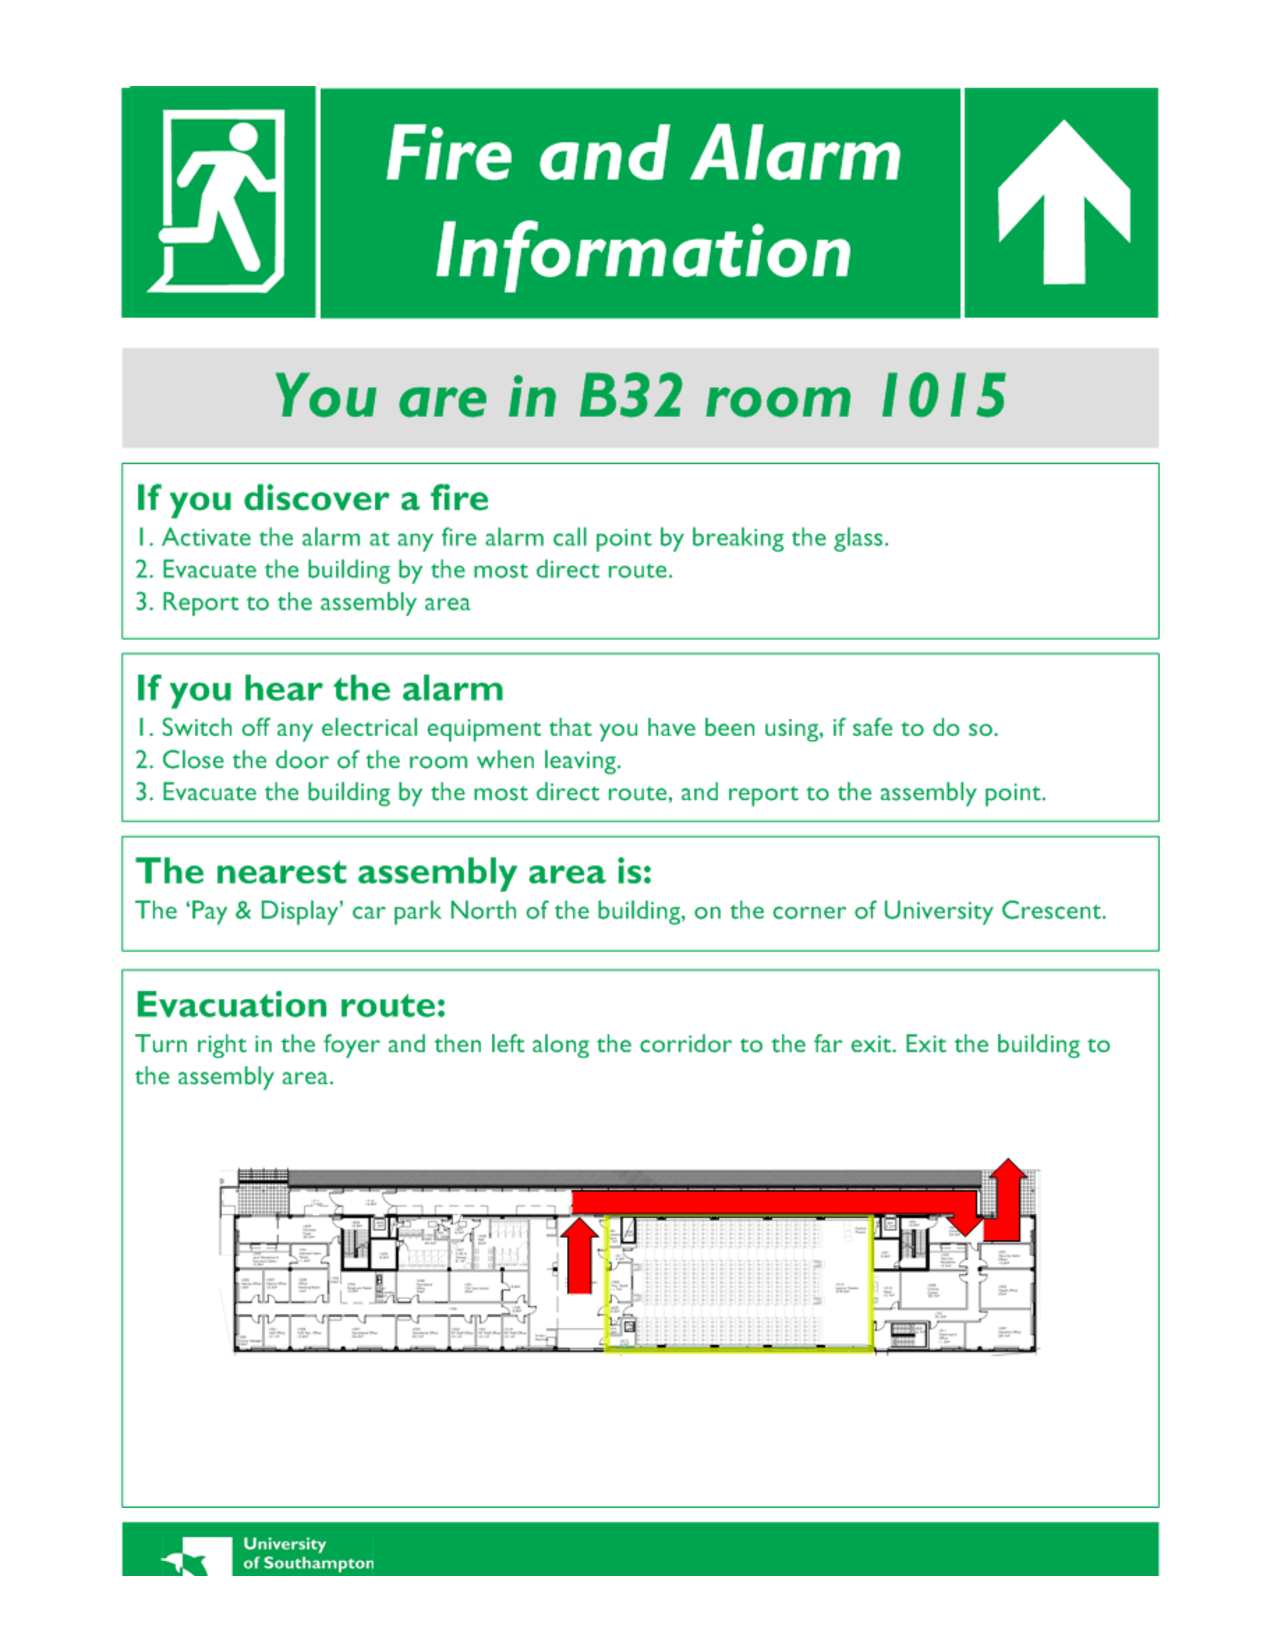
\includepdf[scale=1.0]{FireB32.pdf}
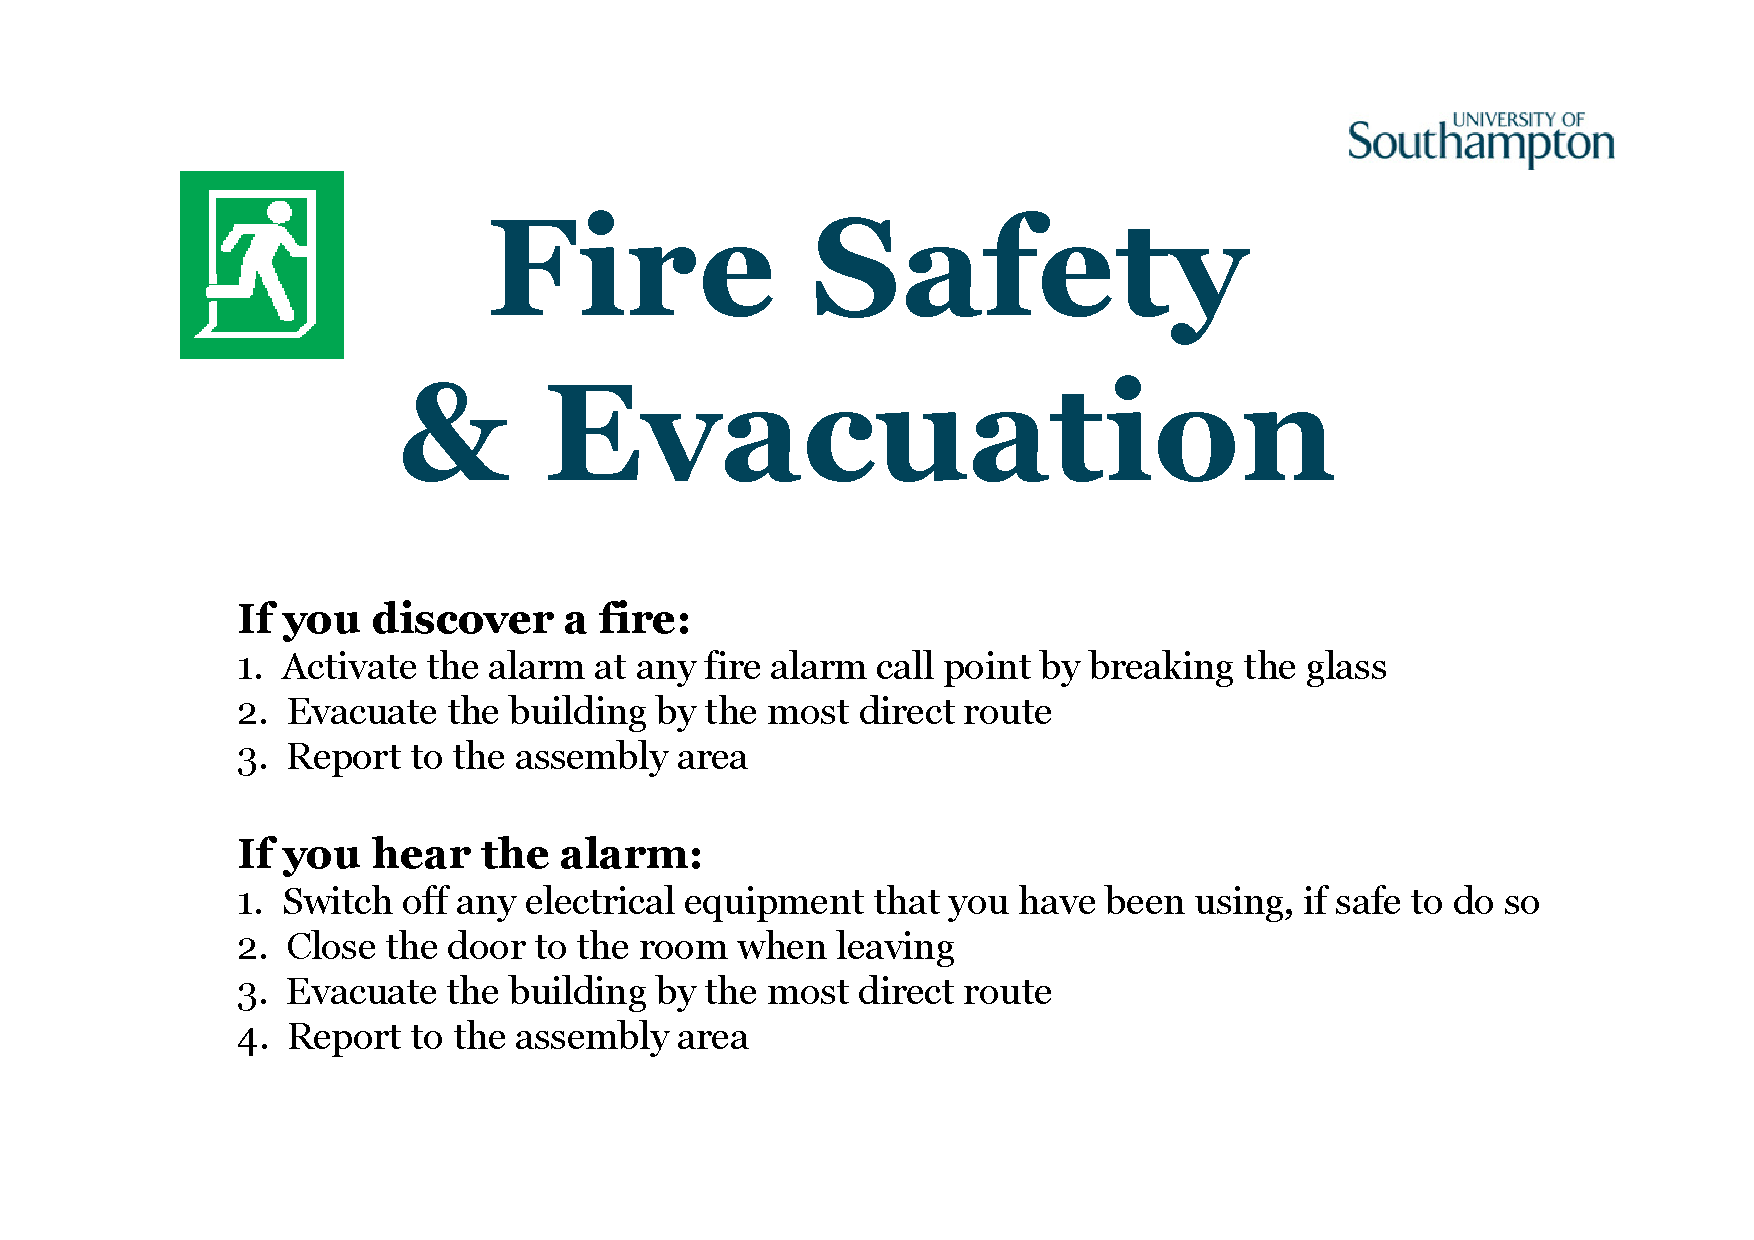
\includepdf[scale=1.0,landscape]{Fire1.pdf}
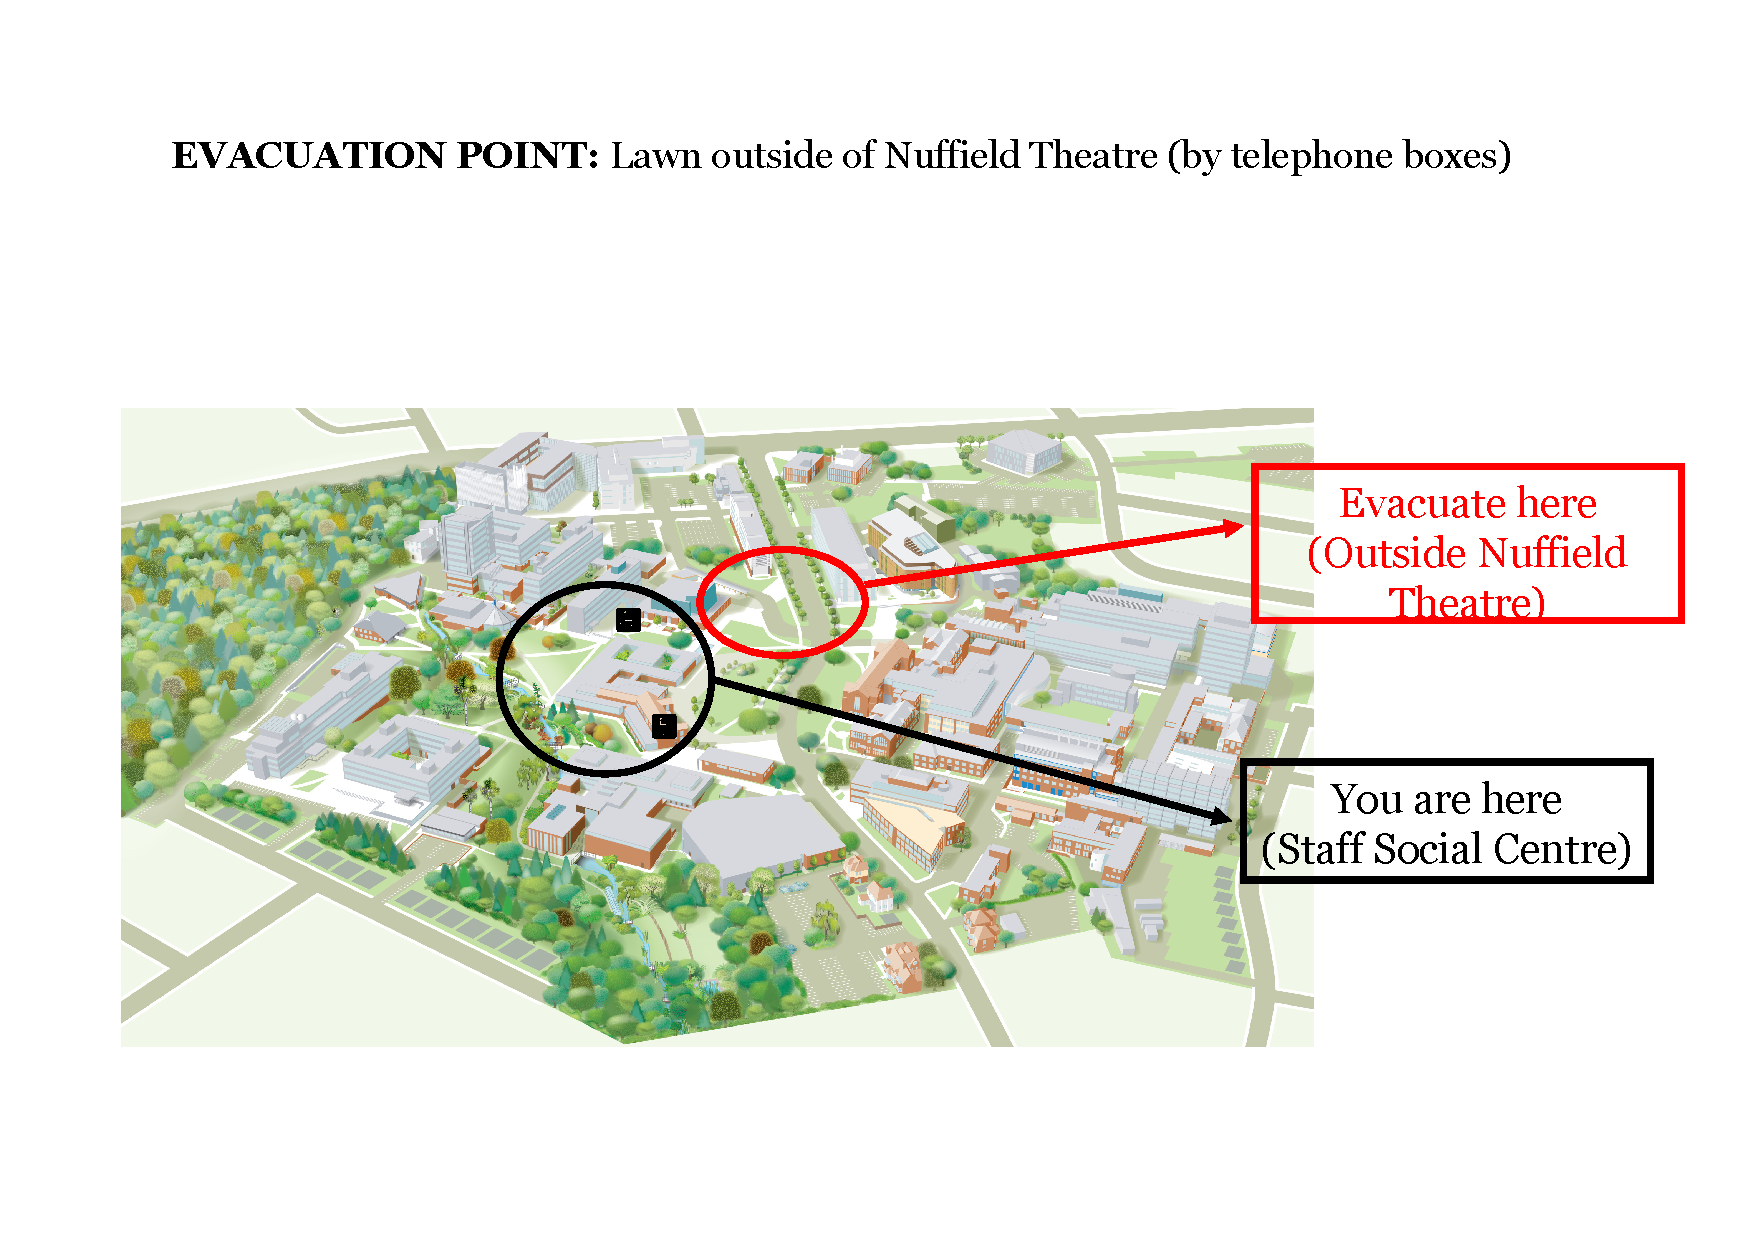
\includepdf[scale=1.0,landscape]{Fire3.pdf}

\end{document}

